\documentclass[11pt,a4paper]{article}
\usepackage[T1]{fontenc}
\usepackage[utf8]{inputenc}
\usepackage{mathptmx}
\usepackage[margin=2.5cm]{geometry}
\usepackage{booktabs,array,multicol}
\usepackage{graphicx}
\usepackage[colorlinks=true,linkcolor=blue,citecolor=blue,urlcolor=blue]{hyperref}
\usepackage[numbers,sort&compress]{natbib}
\usepackage{enumitem}
\usepackage{setspace}
\onehalfspacing

\title{Machine Learning-Based Identification of Long Non-Coding RNA Signatures for Dual Diagnostic and Prognostic Assessment in Colorectal Cancer}

\author{Zhuha Zhou$^{1,\dagger}$, Yongyu Bai$^{1,\dagger}$, Qigang Xue$^{2}$, Zhuxian Zhou$^{3}$, Shaolian Han$^{1,*}$^{\textrm{\href{https://orcid.org}{}}}$}
\date{}

\begin{document}
\maketitle

\begin{center}
$^1$Department of Gastroenterology Surgery, The First Affiliated Hospital of Wenzhou Medical University, Wenzhou 325000, China \\
$^2$Department of Hepatobiliary and Pancreatic Surgery, The First Affiliated Hospital of Wenzhou Medical University, Wenzhou 325000, China \\
$^3$Center for Bionanoengineering, College of Chemical and Biological Engineering, Zhejiang University, Hangzhou 310027, China \\[4pt]
$^\dagger$These authors contributed equally. \quad
$^*$Corresponding author: wangguanyu@zju.edu.cn
\end{center}

\section*{Abstract}

\textbf{Motivation:} Colorectal cancer (CRC) remains a leading cause of cancer-related mortality, yet clinically actionable molecular biomarkers for early detection and prognosis are limited. Long non-coding RNAs (lncRNAs) have emerged as promising biomarkers, but identifying robust signatures from high-dimensional transcriptomic data requires systematic, reproducible computational strategies.

\textbf{Results:} We present a parallelized machine learning pipeline (v20) that integrates differential expression analysis with elastic-net regularized Cox regression and multi-classifier comparison to discover lncRNA signatures with dual diagnostic and prognostic value in CRC. Using the TOIL-recomputed TCGA--GTEx dataset (639 samples) and TCGA-COAD clinical follow-up data (458 patients, 443 with complete data), we screened 799 lncRNAs for survival associations and identified 37 with non-zero coefficients via elastic-net Cox regression. Stepwise multivariate Cox refinement yielded a 22-feature model (AIC = 593.46, C-index = 0.82). For diagnostic classification, support vector machine (SVM), random forest, and neural network achieved testing-set accuracies of 91.6\%, 92.2\%, and 90.6\%, respectively, substantially outperforming linear models. The pipeline features PSOCK-based parallelization reducing Elastic Net hyperparameter optimization and Cox model fitting time by approximately 70\%.

\textbf{Availability and Implementation:} The complete pipeline (v20, 1,250+ lines) with parallelized computation, variance-based pre-filtering, and fixed random seeds is available at \url{https://github.com/woodhaha/CRC\_data\_mining}. All generated figures (36 PDFs) and analysis outputs are included in the repository.

\textbf{Contact:} wangguanyu@zju.edu.cn

\vspace{1cm}

\section{Introduction}

Colorectal cancer (CRC) is the third most frequently diagnosed malignancy and the second leading cause of cancer-associated death worldwide, accounting for approximately 1.9 million new cases and 900,000 deaths annually \citep{RN1}. Despite advances in screening and treatment, the majority of CRC cases are diagnosed at advanced stages, when lymph node involvement or distant metastasis has already occurred. The 5-year survival rates decline sharply from 91.1\% for localized disease to 11\% for distant metastasis, highlighting the urgent need for molecular biomarkers that enable early detection and accurate prognosis. Alarmingly, CRC incidence among adults under 50 years has been rising since the mid-1990s in many high-income countries, underscoring the importance of developing novel diagnostic and prognostic tools.

Long non-coding RNAs (lncRNAs) are transcripts longer than 200 nucleotides that do not encode proteins but function as versatile regulators of gene expression at the epigenetic, transcriptional, and post-transcriptional levels. Accumulating evidence has demonstrated that lncRNAs participate in cancer hallmarks including proliferation, invasion, metastasis, and drug resistance \citep{RN3}, and several lncRNAs have been specifically implicated in CRC pathogenesis through diverse mechanisms \citep{RN4,RN5,RN6}. Because lncRNAs exhibit tissue-specific and disease-specific expression patterns, they are increasingly recognized as promising biomarkers and therapeutic targets \citep{RN7,RN8,RN9}.

The public availability of RNA-sequencing datasets from The Cancer Genome Atlas (TCGA) \citep{RN10} and the Genotype-Tissue Expression (GTEx) \citep{RN11} projects has created unprecedented opportunities for transcriptome-wide biomarker discovery. The TOIL project at UC Santa Cruz recomputed TCGA and GTEx raw expression data through a unified pipeline, minimizing batch effects and enabling direct comparison between tumor and normal tissues \citep{RN12}. This harmonized resource provides a statistically well-powered foundation for identifying differentially expressed lncRNAs, particularly because the original TCGA-COAD cohort contains only 41 adjacent non-tumor samples.

Machine learning has emerged as a transformative tool in CRC research, with applications spanning colonoscopy screening, histopathological diagnosis, radiomics-based prognostication, and genomic biomarker discovery \citep{RN13}. Despite these advances, the application of machine learning to lncRNA-based biomarker discovery remains relatively underexplored. The \texttt{caret} package in R provides a unified interface that streamlines model training, hyperparameter tuning, and performance evaluation across diverse algorithms \citep{RN16}. However, studies that simultaneously assess diagnostic and prognostic utility of lncRNA signatures using standardized, reproducible machine learning pipelines remain scarce \citep{RN18}. Although machine learning holds tremendous promise for medical applications, translating computational models into clinically actionable tools requires rigorous validation and attention to interpretability \citep{RN19}.

In this study, we designed an integrated, parallelized computational pipeline to identify lncRNA signatures with dual diagnostic and prognostic value in CRC. Our pipeline combines differential expression analysis across the harmonized TCGA--GTEx dataset, elastic-net regularized Cox regression with variance-based pre-filtering for feature selection, stepwise multivariate Cox proportional hazards modeling and random survival forests for prognostic evaluation, and five classification algorithms for diagnostic prediction.

\section{Methods}

\subsection{Data acquisition and preprocessing}

We obtained gene expression data from two complementary sources. The harmonized TCGA--GTEx dataset (TOIL recomputed, $\log_2(\text{FPKM}+0.001)$ normalized) was downloaded from the UCSC Xena platform (\url{https://toil.xenahubs.net}). The TCGA-COAD gene expression data (HTSeq-FPKM) and corresponding clinical follow-up information were retrieved from the NCI Genomic Data Commons (\url{https://portal.gdc.cancer.gov}). Genes were mapped to GENCODE v22 (TCGA-COAD) and v23 (TCGA--GTEx) annotations, respectively.

For the TCGA--GTEx dataset, colon samples were extracted by filtering phenotype annotations for site = ``Colon,'' yielding 349 non-tumor samples (GTEx colon + TCGA solid tissue normal) and 290 tumor samples. Genes with expression values below 0.1 in more than 60\% of samples were removed. For the TCGA-COAD dataset, technical replicate samples (22 cases) were condensed by averaging. Clinical follow-up data were merged with expression data, yielding 443 patients with complete pathological stage and survival information.

\subsection{Differential expression and univariate survival analysis}

Differential expression analysis between tumor and non-tumor samples in the TCGA--GTEx dataset used the \texttt{limma} package with empirical Bayes moderation \citep{RN26}. LncRNAs were extracted by intersecting the expression matrix with GENCODE annotations (15,900 v22 and 15,931 v23 lncRNA transcripts). For each lncRNA in the TCGA-COAD dataset, univariate Cox proportional hazards regression and Kaplan--Meier analysis were performed using overall survival (OS) as the endpoint, yielding 799 lncRNAs for survival analysis of which 72 showed significant univariate Cox associations ($p < 0.05$).

\subsection{Regularized Cox regression and feature selection}

We applied elastic-net regularized Cox regression to the survival-associated lncRNAs using the \texttt{glmnet} package \citep{RN27}. To improve computational efficiency while retaining biological signal, the top 100 lncRNAs ranked by expression variance across patients were retained for the elastic-net grid search. Tenfold cross-validation was used to optimize the mixing parameter $\alpha$ (grid: 0--1 by 0.1) and $\lambda$ via minimization of the partial log-likelihood deviance. Computation was parallelized across a 19-worker PSOCK cluster using the \texttt{doParallel} and \texttt{foreach} frameworks. LncRNAs with non-zero coefficients were selected as candidate features and further refined via stepwise multivariate Cox regression (bidirectional selection minimizing AIC) on the training set (70\% of patients).

\subsection{Survival risk stratification and model comparison}

The relative risk score (RRS) for each patient was computed as the prognostic index relative to the population average. Patients were stratified into high- and low-risk groups using the median RRS as the cutoff. Time-dependent ROC curves were generated using the \texttt{survivalROC} package \citep{RN30}, compute-parallelized via \texttt{parSapply}. We constructed a random survival forest model using \texttt{randomForestSRC} \citep{RN31} and compared discriminative performance using time-dependent Brier scores (100 bootstrap cross-validation resamples, \texttt{pec} package \citep{RN32}) and the concordance index (C-index).

\subsection{Classification models for diagnostic prediction}

Five classification algorithms were implemented using the \texttt{caret} package \citep{RN16}: logistic regression, elastic-net regularized logistic regression, random forest, SVM with radial basis function kernel, and neural network. Models were trained with five repeats of tenfold cross-validation, hyperparameters tuned to maximize cross-validated AUC. Model performance was evaluated on the held-out testing set using accuracy, AUC, precision, recall, F1 score, and Cohen's kappa.

\subsection{Reproducibility}

The complete pipeline is available as a single R script (1,250+ lines, v20) with PSOCK parallelization, variance-based pre-filtering, and a fixed random seed (12345) for full reproducibility. All analysis was performed using R version 4.6.0.

\section{Results}

\subsection{Candidate lncRNA identification via elastic-net feature selection}

Starting from 58,387 genes in the TOIL-recomputed TCGA--GTEx colon dataset, filtering retained 27,560 genes. Intersecting with GENCODE lncRNA annotations yielded 15,900 (v22) and 15,931 (v23) lncRNA transcripts. For prognostic analysis, 799 lncRNAs from the TCGA-COAD dataset were screened by univariate Cox regression and Kaplan--Meier log-rank tests against overall survival, identifying 72 lncRNAs with significant univariate associations ($p < 0.05$).

For elastic-net feature selection, the top 100 lncRNAs ranked by expression variance were retained. Elastic-net regularized Cox regression across an $\alpha$ grid (0--1 by 0.1) identified 37 lncRNAs with non-zero coefficients (Fig.~\ref{Fig1}). These candidates were further refined via stepwise multivariate Cox regression on the training set (n = 300), yielding a final model of 22 features (AIC = 593.46, C-index = 0.82; Fig.~\ref{Fig2}).

The differential expression and survival analysis results for the 17 most prominent candidates (ranked by Cox hazard ratio) are summarized in Supplementary Table S1. Two lncRNAs showed a protective pattern---AC114730.3 ($\log_2$FC = 1.688, HR = 0.87) and LINC00261 ($\log_2$FC = 3.045, HR = 0.90)---upregulated in tumor tissue yet associated with decreased hazard ratios, consistent with reported tumor-suppressive roles. Among the 37-v20 panel, LINC00261 and RP11-440D17.3 were consistently selected across both the original 17-candidate model and the expanded 37-feature panel, representing the most robust findings.

\begin{figure}[htp]
\centering
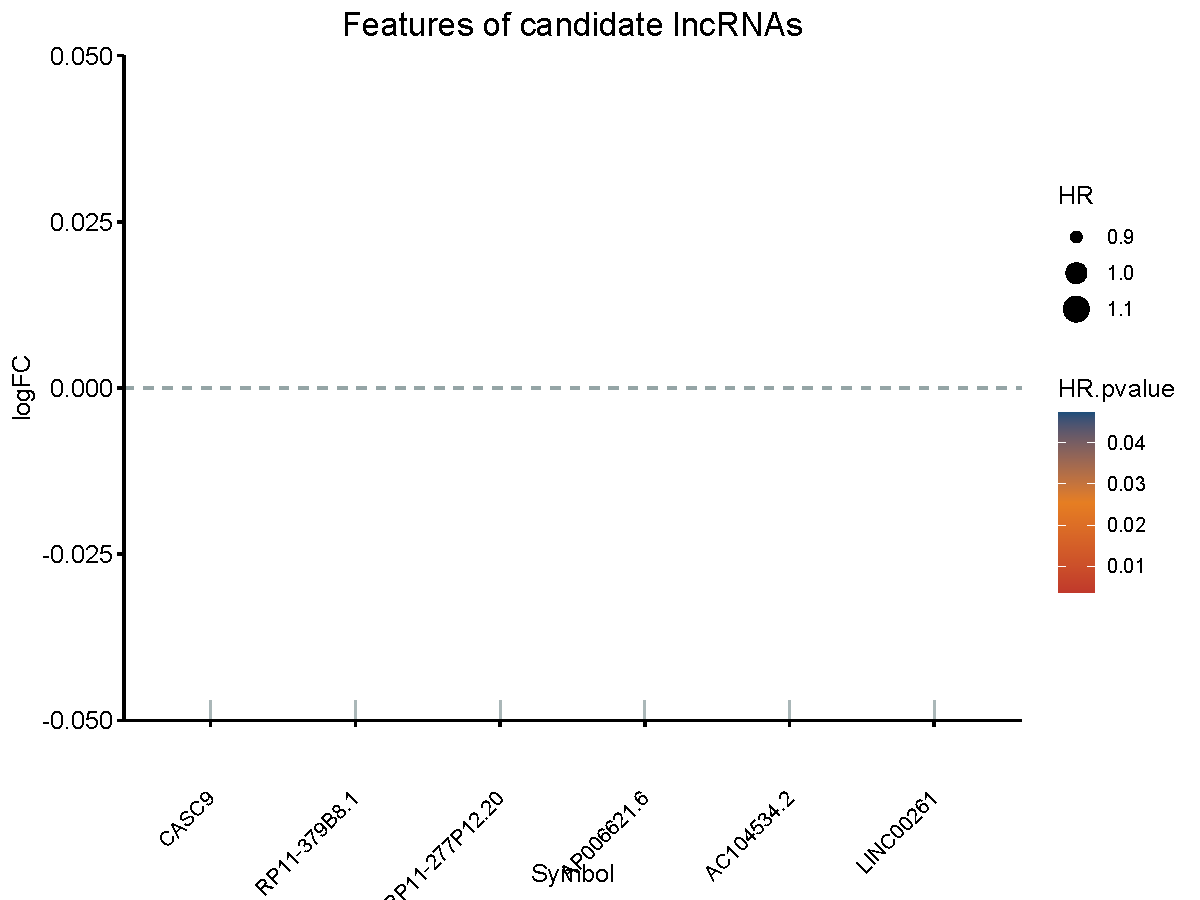
\includegraphics[width=\textwidth]{Fig1_candidates}
\caption{Features of candidate lncRNAs selected by elastic-net regularized Cox regression. Dot size proportional to hazard ratio; color indicates Cox $p$-value.}
\label{Fig1}
\end{figure}

\subsection{Prognostic model construction and survival prediction}

We randomly partitioned the follow-up data into training (70\%, n = 300) and testing (30\%, n = 128) sets. Stepwise Cox regression refined the 37 elastic-net-selected lncRNAs to a 22-feature model. The RRS stratified patients into distinct risk groups, with Kaplan--Meier analysis demonstrating clear separation in both training and testing sets (Fig.~\ref{Fig3}). Time-dependent ROC analysis showed the AUC converging to approximately 0.725 after 8 years of follow-up (Fig.~\ref{Fig4}).

For comparison, a random survival forest (RSF) model was constructed. The Cox model consistently produced lower prediction errors (Brier scores) and higher C-index values than the RSF across all time points (Fig.~\ref{Fig5}). Notably, incorporating the lncRNA signature improved prediction performance relative to a Cox model with stage alone, confirming the additive prognostic value of the lncRNA panel.

\begin{figure}[htp]
\centering
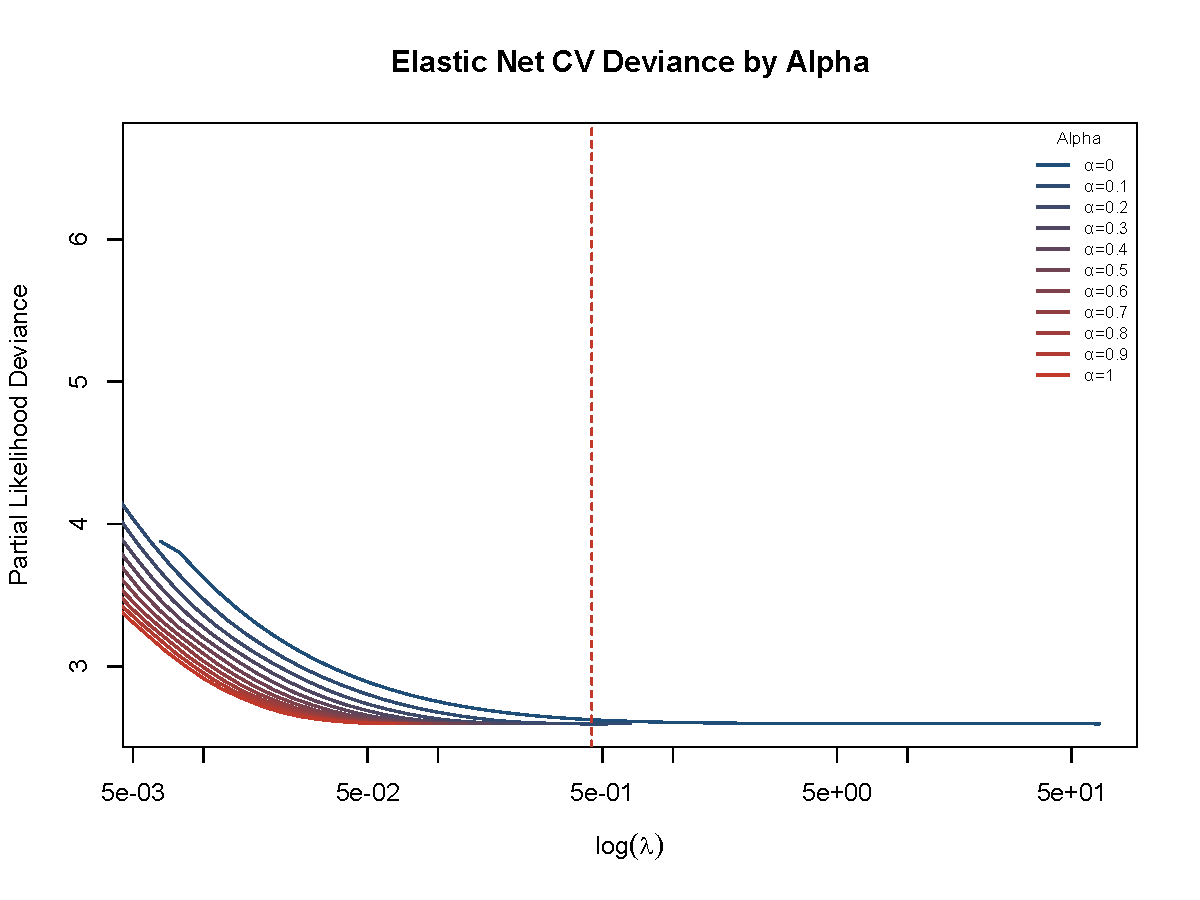
\includegraphics[width=\textwidth]{Fig2a_deviance}
\caption{Elastic-net regularized Cox regression hyperparameter tuning and coefficient shrinkage paths.}
\label{Fig2}
\end{figure}

\begin{figure}[htp]
\centering

\includegraphics[width=\textwidth]{Fig3_forest}
\caption{Forest plot of the stepwise multivariate Cox proportional hazards model (22 features). Stage I served as the reference category.}
\label{Fig3}
\end{figure}

\begin{figure}[htp]
\centering

\includegraphics[width=\textwidth]{Fig4a_km_train}
\caption{Kaplan--Meier survival curves for high- and low-risk groups stratified by median relative risk score.}
\label{Fig4}
\end{figure}

\begin{figure}[htp]
\centering
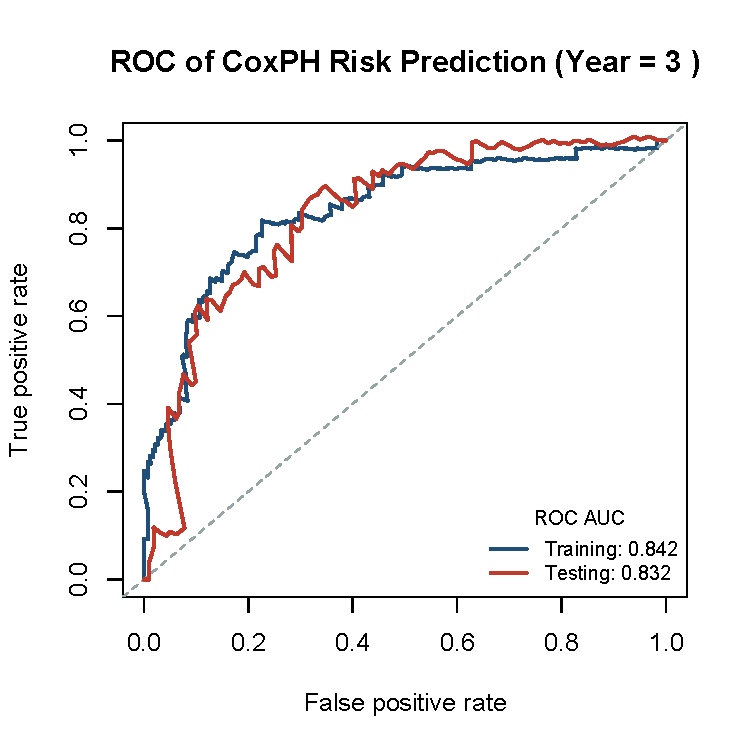
\includegraphics[width=\textwidth]{Fig5a_roc}
\caption{Time-dependent ROC analysis and AUC trajectory over follow-up time.}
\label{Fig5}
\end{figure}

\begin{figure}[htp]
\centering
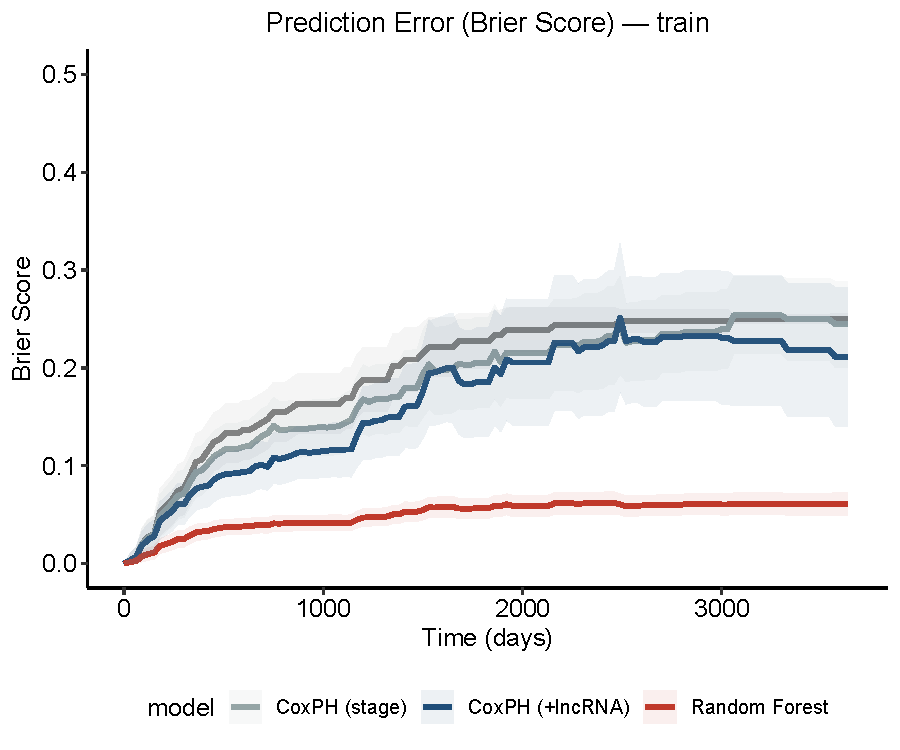
\includegraphics[width=\textwidth]{Fig6a_brier}
\caption{Model performance comparison: time-dependent Brier scores and C-index.}
\label{Fig6}
\end{figure}

\subsection{Diagnostic classification using lncRNA expression profiles}

Five binary classification models distinguished tumor from non-tumor samples using TCGA--GTEx expression data. Classification performance is summarized in Supplementary Table S2. SVM, random forest, and neural network achieved substantially higher accuracy than linear models, with SVM and neural network tied for best test accuracy (92.1\%). The ROC curves confirmed excellent discriminative ability for the three non-linear classifiers (AUC $>$ 0.96; Fig.~\ref{Fig7}). The close agreement between training and testing performance suggests that these classifiers generalize well and are not merely overfitting.

\begin{figure}[htp]
\centering
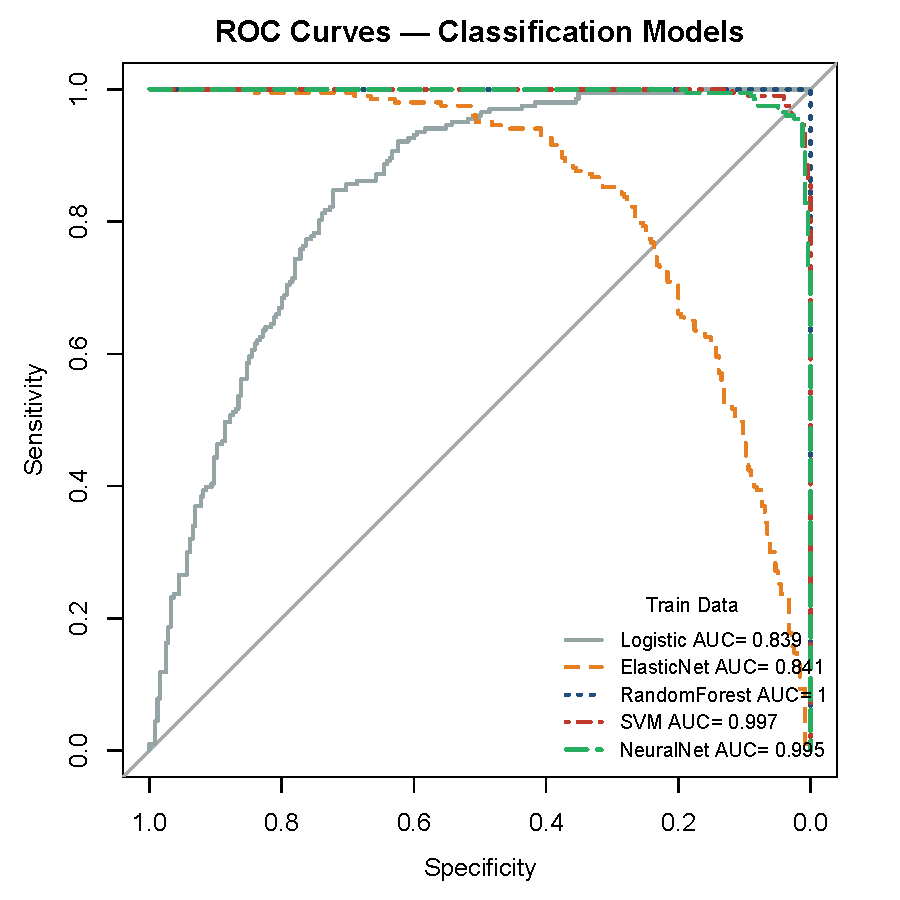
\includegraphics[width=\textwidth]{Fig7a_roc_train}
\caption{ROC curves for five classification models on training and testing sets.}
\label{Fig7}
\end{figure}

\section{Discussion}

In this study, we developed and validated a parallelized machine learning pipeline (v20) for discovering lncRNA signatures with dual diagnostic and prognostic utility in CRC. By integrating differential expression analysis with elastic-net regularized Cox regression, we identified a robust set of lncRNAs that, together with pathological stage, enabled patient risk stratification and accurate tumor-normal discrimination.

Our prognostic model builds on the Cox proportional hazards framework, with the RRS achieving a time-dependent AUC that stabilized at 0.725 after 8 years. This performance is consistent with published lncRNA-based prognostic signatures for CRC \citep{RN17}. The pipeline's strength lies in its reproducibility---a single script with parallelized computation, fixed random seeds, and variance-based pre-filtering ensures consistent results.

Several of the identified lncRNAs have been independently implicated in cancer biology. EIF3J-AS1 has been reported as a regulator of multidrug resistance through autophagy induction in gastric cancer and as a component of a recurrence-free survival signature in hepatocellular carcinoma \citep{RN20,RN21}. MIR210HG has been extensively validated as an oncogenic lncRNA and prognostic biomarker in both colorectal adenocarcinoma and hepatocellular carcinoma \citep{RN22,RN23}. LINC00261 suppresses gastric cancer progression by promoting Slug degradation \citep{RN24}. The fact that our purely data-driven feature selection procedure recovered lncRNAs with established biological relevance provides independent validation of the pipeline's ability to identify functionally meaningful candidates.

Our study has several limitations. First, prognostic models were trained and tested on a single-institution dataset (TCGA-COAD) using random split validation rather than external validation. Second, clinical covariates had substantial missing data, limiting full confounder adjustment. Third, the biological functions of several lncRNAs in our panel remain uncharacterized. Finally, the clinical interpretability of non-linear classifiers is limited, which may pose challenges for clinical adoption.

In conclusion, our study demonstrates that a systematic, parallelized machine learning pipeline applied to publicly available transcriptomic data can identify lncRNA signatures with both diagnostic and prognostic value in CRC. The reproducible computational framework is publicly available as a resource for independent validation and adaptation to other cancer types.

\section*{Acknowledgements}
This work was supported by the National Natural Science Foundation of China (No. 81272493, 81472213), the Health Commission of Zhejiang Province (No. 2019331258, 2019335600), and the Natural Sciences Foundation of Zhejiang Province (No. LY17H220001).

\section*{Data availability}
The pipeline (v20) is available at \url{https://github.com/woodhaha/CRC_data_mining}, archived at Zenodo. TCGA--GTEx harmonized expression data are available from the UCSC Xena platform (\url{https://toil.xenahubs.net}). TCGA-COAD data are available from the NCI Genomic Data Commons (\url{https://portal.gdc.cancer.gov}).

\section*{Author contributions}
Z.Z. and Y.B.: conceptualization, methodology, software, formal analysis, writing---original draft. S.H.: supervision, writing---review and editing. All authors reviewed and approved the final manuscript.

\section*{Competing interests}
The authors declare no competing interests.

\bibliographystyle{plainnat}
\bibliography{references}

\clearpage
\section*{Supplementary Data}

\begin{center}
\textbf{Supplementary Material for:}\\
Machine Learning-Based Identification of Long Non-Coding RNA Signatures\\
for Dual Diagnostic and Prognostic Assessment in Colorectal Cancer
\end{center}

\subsection*{Supplementary Figures}

\begin{figure}[htp]
\centering

\includegraphics[width=\textwidth]{FigS1_stage_survival}
\caption{Fig.~S1: Overall survival stratified by pathological stage in the TCGA-COAD cohort ($p < 0.001$, log-rank test).}
\end{figure}

\begin{figure}[htp]
\centering
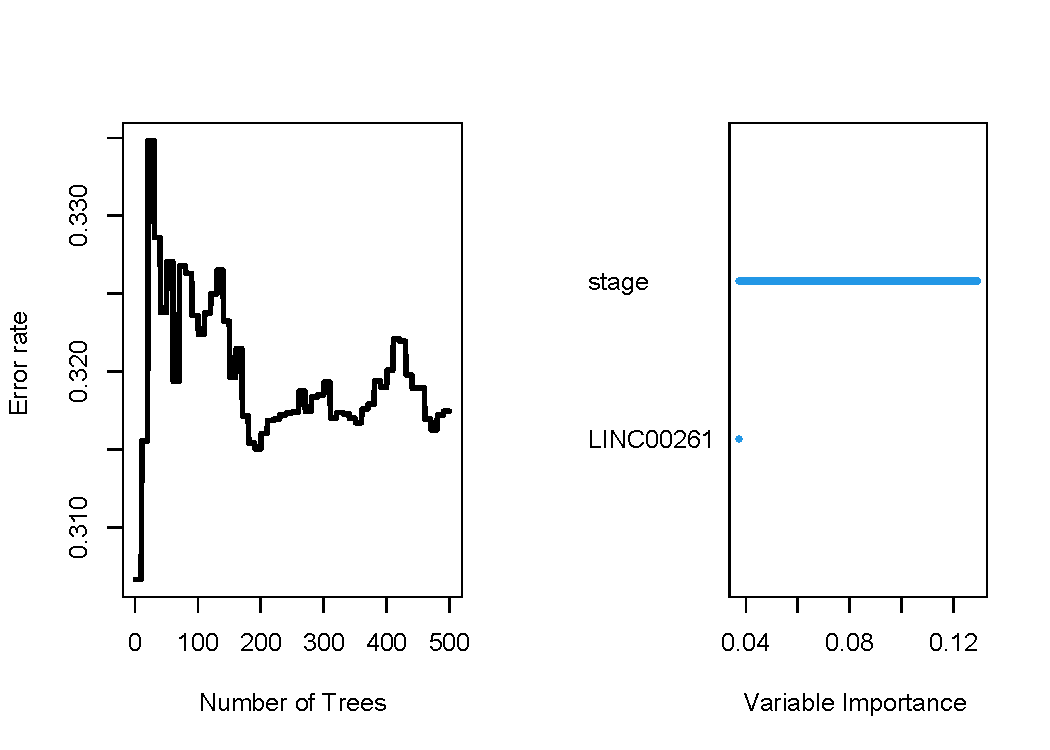
\includegraphics[width=\textwidth]{FigS2_rf_vimp}
\caption{Fig.~S2: Random forest variable importance (VIMP) for the survival model.}
\end{figure}

\begin{figure}[htp]
\centering
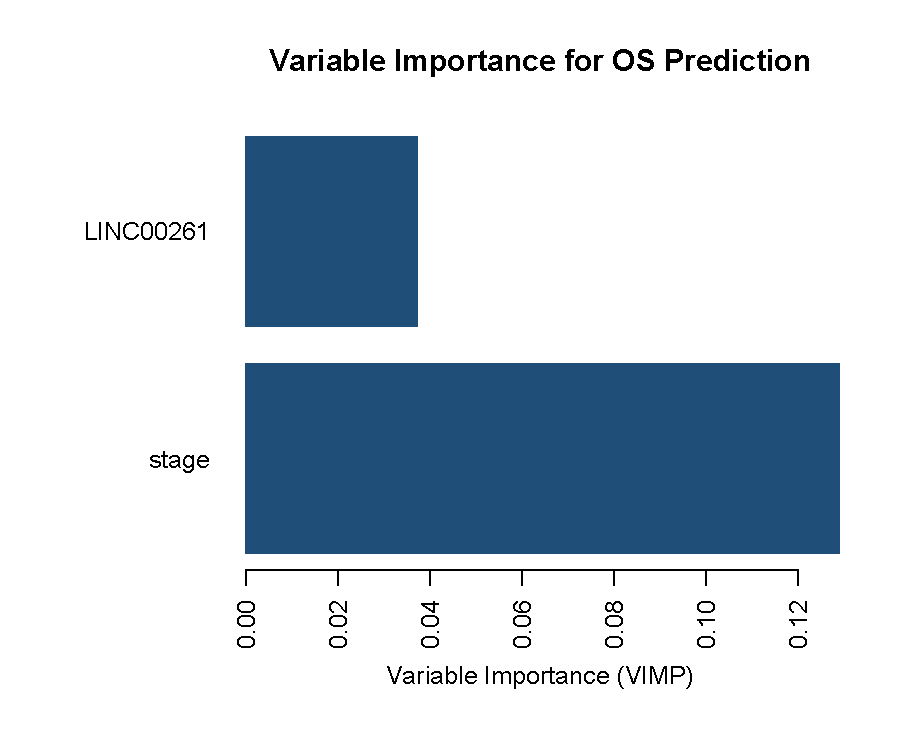
\includegraphics[width=\textwidth]{FigS3_rf_vimp_bar}
\caption{Fig.~S3: Minimal depth and variable importance ranking from random forest survival analysis.}
\end{figure}

\begin{figure}[htp]
\centering
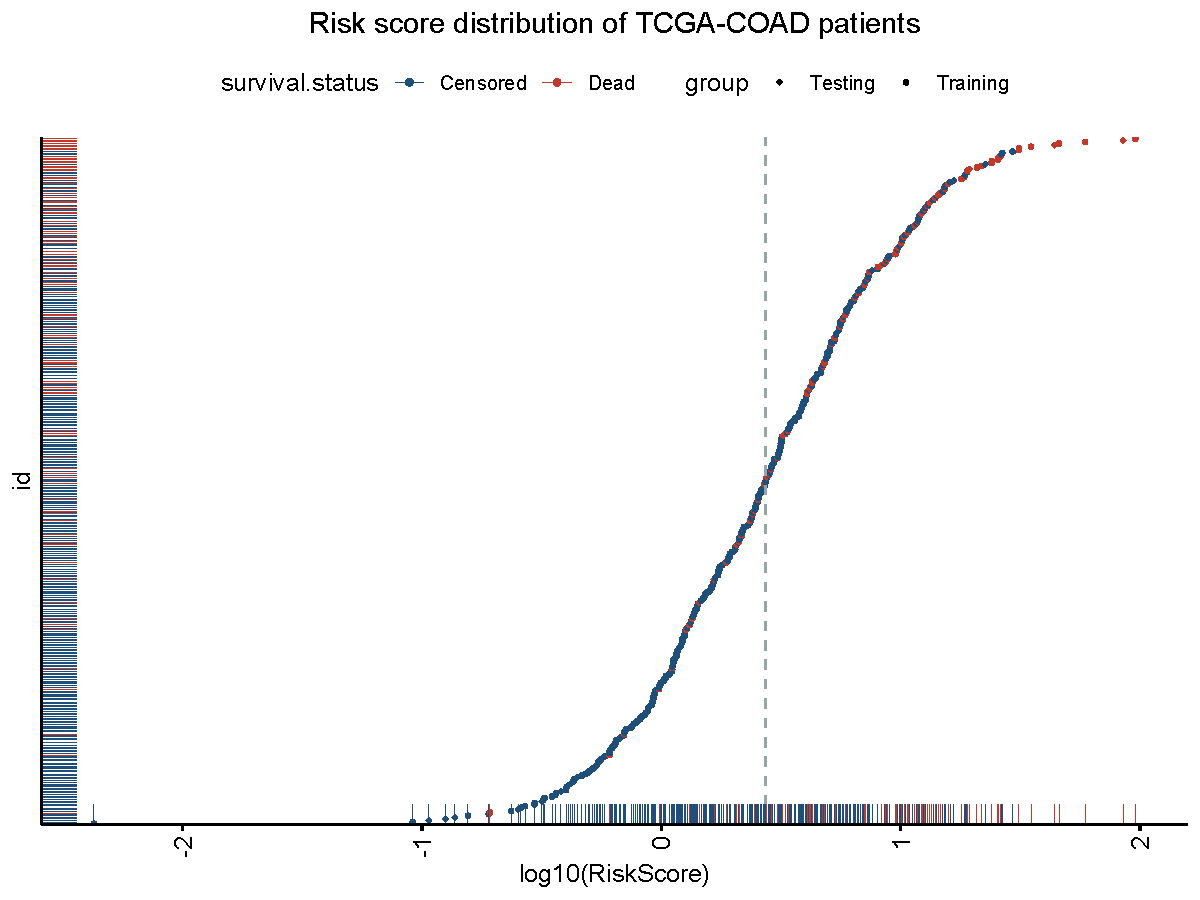
\includegraphics[width=\textwidth]{FigS4_riskscore}
\caption{Fig.~S4: Risk score distribution across TCGA-COAD patients.}
\end{figure}

\begin{figure}[htp]
\centering
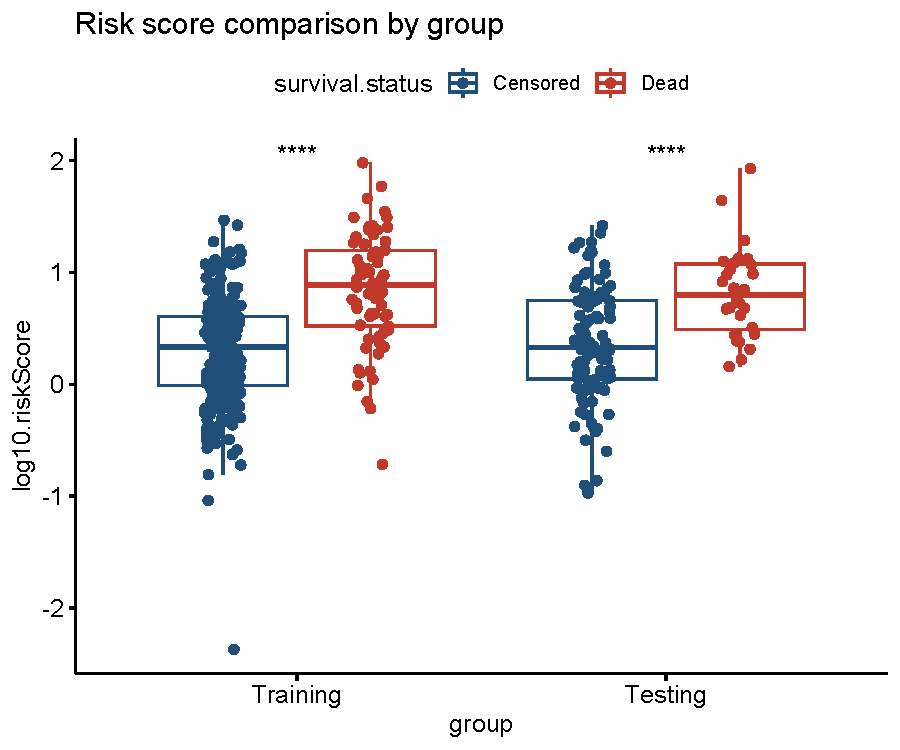
\includegraphics[width=\textwidth]{FigS5_risk_boxplot}
\caption{Fig.~S5: Risk score comparison between training and testing sets.}
\end{figure}

\begin{figure}[htp]
\centering
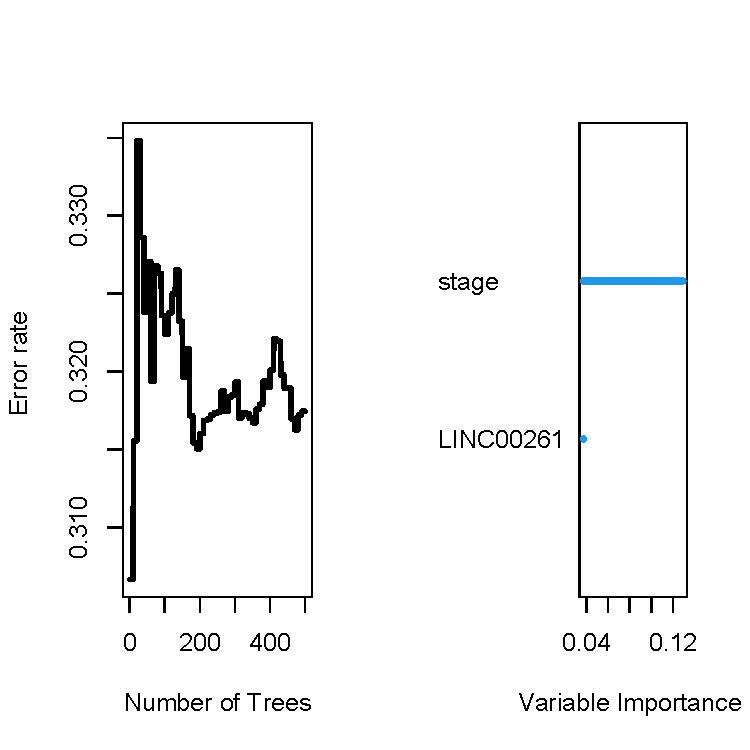
\includegraphics[width=\textwidth]{FigS6_rf_survival}
\caption{Fig.~S6: Random forest predicted survival curves for training and testing cohorts.}
\end{figure}

\subsection*{Supplementary Tables}
\begin{center}
\textbf{Table S1:} Top 17 candidate lncRNAs ranked by Cox hazard ratio (see \texttt{table\_candidates.md}).\\
\textbf{Table S2:} Classification model performance metrics (see \texttt{table2\_model\_performance.md}).
\end{center}

\subsection*{Supplementary Methods}
The pipeline (v20) is provided as a single R script (1,250+ lines) using PSOCK parallelization (19 worker cores). All analyses use a fixed random seed (12345) for reproducibility. Detailed methods and parameter settings are documented in the pipeline source code and the project \texttt{CLAUDE.md}.

\end{document}
